\section{Absorption models and the method of characteristics}
\label{sec:moc}

In previous work we have been able to describe the birth--death dynamics of
pathogenic particles inside a host cell that can rupture. We now wish to extend that
understanding to cases in which several host cells share a medium, and this requires
deciding what happens when the first of them ruptures. The shared medium suddenly
gains a potentially large cohort of pathogenic particles, available for subsequent
absorption by the remaining hosts.

The analysis so far has assumed \emph{immediate transfer}: the entire pathogenic
contents of a rupturing cell relocate at once to the interior of another host. That
is a strong assumption. A more realistic alternative is an \emph{absorption period}:
following a rupture, absorption events redistribute the released cohort among the
remaining hosts, and only when every particle has been taken up do birth, death and
rupture resume. Working towards such absorption models, we begin with the case in
which a pathogenic cohort infiltrates a single host cell.

Three models are treated in increasing order of difficulty. In the first two the
particles are conserved or only lost, the state space is finite, and an independence
argument delivers the generating function without any need to solve a partial
differential equation. In the third, replication inside the host opens an infinite
state space and the independence shortcut fails, so the PDE must be confronted
directly. The method of characteristics is developed on the second model, where the
answer is already known, and then applied to the third.

\subsection{Absorption only}
\label{sec:absonly}

The simplest absorption process has a single host cell that takes in pathogenic
particles, with no subsequent dynamics --- no birth and no death of pathogen within
the host.

Introduce $\xt$ and $\yt$ for the number of pathogenic particles inside and outside
the host cell respectively; the same labelling is used for every version of the
single-host model below. Events are assumed stochastic, with exponentially
distributed inter-event times, a property that follows from the assumption that
event rates do not depend on time. The continuous-time stochastic process
$\{(\xt,\yt) : t\in[0,\infty)\}$ therefore has the memoryless Markov property.

With only absorption to consider, the model is specified by the following
outcome-likelihoods over an infinitesimal duration $\Delta t$, taken in the limit to
zero:
\begin{align*}
     \pr{\Delta\xx= 1,\;\Delta\yy = -1 \;|\; \yt = j} &= j \alpha \Delta t,  &&\text{(absorption)}\\
     \pr{\Delta\xx= 0,\;\Delta\yy = 0 \;|\; \yt = j} &= 1 -  j \alpha \Delta t,  &&\text{(no event)}
\end{align*}
where $\Delta\xx = \xx_{t+\Delta t}-\xt$, and similarly for $\yy$. Note the factor
$j$: each of the extracellular particles is independently subject to the same
probability $\alpha\Delta t$ of being taken up. The initial condition is
$\xx_0 = 0$, $\yy_0 = N$ --- a starter population of census $N$ occupying the
extracellular medium.

Defining state probabilities $\pt = \pr{\xt=i,\ \yt=j}$, the forward Kolmogorov
equations are
\begin{equation}
\label{F1}
\ddt{\p} = \alpha(j+1)p_{i-1,j+1} - \alpha j\,\p .
\end{equation}
With the probability generating function
\begin{equation}
\label{pgfDef}
G(x,y,t) = \sum_i\sum_j \pt\, x^iy^j
\;\;\lrb{=\mathbb{E}\bigl[x^{\xt}y^{\yt}\bigr]},
\end{equation}
we can convert \cref{F1} into a PDE. Multiply each equation by $x^iy^j$,
\begin{equation*}
\pddt{\p x^iy^j} = \alpha(j+1)p_{i-1,j+1}x^iy^j - \alpha j\,\p x^iy^j ,
\end{equation*}
and sum over $i$ and $j$ for non-zero $\pt$:
\begin{equation}
\label{pdeDere2}
\sum_{i = 0}^N\sum_{j=0}^N\pddt{\p x^iy^j} = \alpha\sum_{i = 1}^{N+1}\sum_{j=-1}^{N-1}(j + 1) p_{i-1,j+1}x^iy^j - \alpha \sum_{i = 0}^N\sum_{j=0}^Nj \p x^iy^j.
\end{equation}
(The sums are finite because $\pt=0$ for all $t$ whenever $i+j\neq N$: pathogenic
particles in this model are neither created nor destroyed.) Shifting indices in the
first double sum and rearranging,
\begin{equation*}
\sum_{i = 0}^N\sum_{j=0}^N\pddt{\p x^iy^j} = \alpha\left(x\sum_{i = 0}^N\sum_{j=0}^N j p_{i,j}x^{i}y^{j-1} -  y\sum_{i = 0}^N\sum_{j=0}^Nj \p x^iy^{j-1} \right),
\end{equation*}
which is a statement about partial derivatives,
\begin{equation*}
\sum_{i = 0}^N\sum_{j=0}^N\pddt{\p x^iy^j} = \alpha\left(x - y\right)\sum_{i = 0}^N\sum_{j=0}^N \pdd{\p x^iy^j}{y}.
\end{equation*}
Recognising \cref{pgfDef},
\begin{equation}
\label{PDE1}
\pddt{G(x,y,t)} = \alpha\left(x - y\right) \pdd{G(x,y,t)}{y},
\qquad G(x,y,0) = y^N .
\end{equation}

This first-order linear initial value problem proves surprisingly awkward. The
method of characteristics, though applicable in principle to equations in three
variables, led at first only to mystification. As it happens, the solution can be
obtained by other means, and it is worth doing so both because the answer is needed
and because it provides a check on the characteristics machinery developed in
\cref{sec:mocabsdeath}.

\subsubsection*{Exploiting independence}

The function $G$ above was specific to $\xx_0=0$, $\yy_0=N$. Define more generally
\begin{equation*}
G_n(x,y,t) = \sum_i\sum_j \pr{\xt = i,\;\yt=j \;|\;\xx_0 = 0,\;\yy_0=n } x^i y^j .
\end{equation*}
In a process of pure absorption the $N$ particles are taken up one by one, and if we
follow a single particle its behaviour does not depend on the movements of its
neighbours. Because of this independence, $\xt$ and $\yt$ decompose into sums of
$n$ single-particle variables,
\begin{align*}
\xt &= \xt^{(1)} + \xt^{(2)} + \dots + \xt^{(n)},\\
\yt &= \yt^{(1)} + \yt^{(2)} + \dots + \yt^{(n)},
\end{align*}
from which
\begin{equation}
\label{indRelPGF}
G_n(x,y,t) = \bigl(G_1(x,y,t)\bigr)^n ,
\end{equation}
since
\begin{align*}
G_n(x,y,t) &= \ex{x^{\sum_{k=1}^n \xt^{(k)}} y^{\sum_{k=1}^n \yt^{(k)}}}
= \ex{\prod_{k=1}^n x^{\xt^{(k)}} \prod_{k=1}^n y^{\yt^{(k)}}}\\
&= \prod_{k=1}^n\ex{x^{\xt^{(k)}} y^{\yt^{(k)}}}
= \bigl(G_1(x,y,t)\bigr)^n .
\end{align*}

Now consider a single initial particle, $\xx_0=0$, $\yy_0=1$. It is eventually
absorbed, and that is the final state of the system: no other states are reachable,
so $\pt=0$ for all $t$ whenever $i+j\neq1$. The forward Kolmogorov equations reduce
to
\begin{align*}
\ddt{p_{0,1}(t)} = -\alpha p_{0,1}(t), && \ddt{p_{1,0}(t)} = \alpha p_{0,1}(t),
\end{align*}
giving
\begin{align*}
p_{0,1}(t) = \ee^{-\alpha t}, && p_{1,0}(t) = 1 - \ee^{-\alpha t} .
\end{align*}

\begin{figure}[H]
\centering
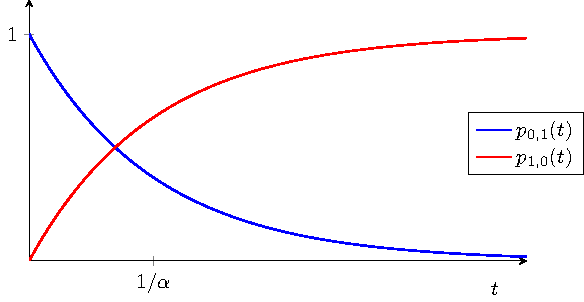
\includegraphics[width = 0.62\textwidth]{figures/IMG_ch3/abs1.pdf}
\caption{State probabilities for the single-particle absorption-only model. The
particle begins outside the cell ($p_{0,1}$, decaying exponentially at rate $\alpha$)
and ends inside it ($p_{1,0}$). There is nowhere else for it to go, so the two
curves sum to one at every time.}
\label{fig:abs1}
\end{figure}

These being the only two non-zero state probabilities of the single-particle system,
\begin{align*}
G_1(x,y,t) &= p_{1,0}(t)\,x + p_{0,1}(t)\,y
= \lrb{1-\ee^{-\alpha t}}x + \ee^{-\alpha t}y ,
\end{align*}
and applying \cref{indRelPGF} gives the generating function for any initial census,
\begin{equation}
\label{eq:Gabsonly}
G_n(x,y,t) = \Bigl(\lrb{1-\ee^{-\alpha t}}x + \ee^{-\alpha t}y\Bigr)^n .
\end{equation}
This does satisfy \cref{PDE1} together with its initial condition
$G_n(x,y,0) = y^n$. The form is recognisable: $\xt\sim\text{Binomial}(n,1-\ee^{-\alpha t})$,
as it must be, since the $n$ particles are absorbed independently and each has been
taken up by time $t$ with probability $1-\ee^{-\alpha t}$.

\subsection{Absorption--death}
\label{sec:absdeath}

In reality a pathogenic particle resident in a host cell may die. Keeping $\xt$ and
$\yt$ for the intracellular and extracellular counts, death is incorporated as
follows:
\begin{align*}
     \pr{\Delta\xx= 1,\;\Delta\yy = -1 \;|\; \yt = j} &= j \alpha \Delta t,  &&\text{(absorption)}\\
      \pr{\Delta\xx= -1,\;\Delta\yy = 0 \;|\; \xt = i} &= i \mu \Delta t,  &&\text{(death)}\\
     \pr{\Delta\xx= 0,\;\Delta\yy = 0 \;|\; \yt = j,\, \xt=i} &= 1 -  \lrb{ j\alpha + i\mu}\Delta t,  &&\text{(no event)}
\end{align*}
with forward Kolmogorov equations
\begin{equation}
\label{FK1}
\ddt{\p} = \alpha(j+1)p_{i-1,j+1} + \mu(i+1)p_{i+1,j} - (\alpha j + \mu i)\p .
\end{equation}
An analogous derivation to that of \cref{sec:absonly} leads to the first-order
linear PDE
\begin{equation}
\label{PDE2}
\pddt{G(x,y,t)} = \mu(1-x)\pdd{G(x,y,t)}{x} + \alpha\left(x - y\right)\pdd{G(x,y,t)}{y},
\qquad G(x,y,0)=y^N,
\end{equation}
and the same familiar difficulty. But once again the solution can be constructed via
\cref{indRelPGF}, since individual particles remain independent in their movements.

Without birth events the number of particles cannot exceed its initial value, so for
an isolated particle the generating function has just three terms,
\begin{equation*}
G_1(x,y,t) = p_{0,0}(t) + p_{1,0}(t)\,x + p_{0,1}(t)\,y .
\end{equation*}
The state probabilities follow from
\begin{align*}
\ddt{p_{0,1}(t)} = -\alpha p_{0,1}(t), && \ddt{p_{1,0}(t)} = \alpha p_{0,1}(t) - \mu p_{1,0}(t),
\end{align*}
whence
\begin{align}
\label{eq:absdeathstates}
p_{0,1}(t) = \ee^{-\alpha t}, &&
p_{1,0}(t) = \frac{\alpha}{\mu - \alpha}\Bigl(\ee^{-\alpha t} - \ee^{-\mu t}\Bigr), &&
p_{0,0}(t) = 1 - p_{0,1}(t) - p_{1,0}(t).
\end{align}

\begin{figure}[H]
\centering
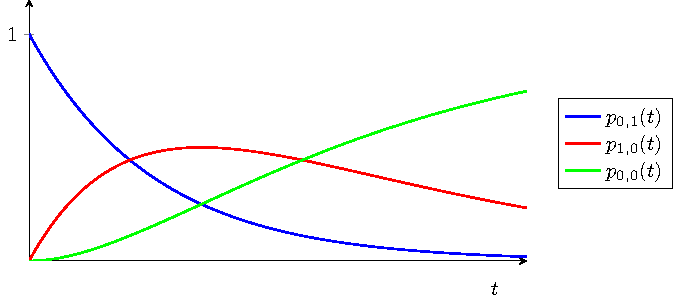
\includegraphics[width = 0.62\textwidth]{figures/IMG_ch3/abs2.pdf}
\caption{State probabilities for the single-particle absorption--death model,
\cref{eq:absdeathstates}. The particle starts outside ($p_{0,1}$, blue), is absorbed
into the cell ($p_{1,0}$, red, which rises and then decays as death takes over), and
finally dies ($p_{0,0}$, green, absorbing).}
\label{fig:abs2}
\end{figure}

Applying \cref{indRelPGF} gives the general generating function
\begin{equation}
\label{eq:Gabsdeath}
G_n(x,y,t) = \Bigl(1-\tfrac{\mu}{\mu - \alpha}\ee^{-\alpha t} + \tfrac{\alpha}{\mu - \alpha}\ee^{-\mu t}
+ \tfrac{\alpha}{\mu - \alpha}\bigl(\ee^{-\alpha t} - \ee^{-\mu t}\bigr)x + \ee^{-\alpha t}y\Bigr)^n .
\end{equation}

\subsection{The method of characteristics, tested on absorption--death}
\label{sec:mocabsdeath}

Before continuing to absorption--birth--death, where replication may occur within
the host cell and the independence shortcut is unavailable, it is worth revisiting
absorption--death from the point of view of its PDE. Having \cref{eq:Gabsdeath}
already in hand makes this an ideal test case.\footnote{I am grateful to Benjamin
Sharp for the advice on how to apply the method of characteristics to three-variate
problems that unlocked this section.}

Introduce a change of variables $(x,y,t)\to(s,r,\tau)$,
\begin{equation*}
G(x,y,t) = G\bigl(x(s,r,\tau),\,y(s,r,\tau),\,t(s,r,\tau)\bigr) \equiv G(s,r,\tau).
\end{equation*}
The method works by seeking solutions along the characteristic curves of constant
$s$ and $r$, on which $G$ is a function of $\tau$ alone. To fix the parametrisation
we impose an initial surface,
\begin{equation}
\label{ICpar}
x(s,r,0) = s, \qquad y(s,r,0) = r, \qquad t(s,r,0) = 0 .
\end{equation}
With $G$ a function of $\tau$ only along a characteristic, the chain rule gives
\begin{equation*}
\dda{G}{\tau} = \pddt{G}\dda{t}{\tau} + \pdd{G}{x}\dda{x}{\tau} + \pdd{G}{y}\dda{y}{\tau},
\end{equation*}
which is to be compared with \cref{PDE2} written as
\begin{equation*}
0 = -\pddt{G} + \mu(1-x)\pdd{G}{x} + \alpha(x-y)\pdd{G}{y} .
\end{equation*}
Comparing coefficients yields the characteristic system
\begin{align}
\dda{G}{\tau} &= 0, \label{ch11}\\
\dda{t}{\tau} &= -1, \label{ch12}\\
\dda{x}{\tau} &= \mu(1-x), \label{ch13}\\
\dda{y}{\tau} &= \alpha(x-y). \label{ch14}
\end{align}

\paragraph{The equation for $G$, \eqref{ch11}.}
$G$ is constant along characteristics, $G = \phi(s,r)$. Under \cref{ICpar} the
initial condition $G(x,y,0)=y^N$ becomes $G(s,r,0)=r^N$, so $\phi(s,r)=r^N$ and
\begin{equation}
\label{GrN}
G(s,r,\tau) = r^N .
\end{equation}
The whole problem thus reduces to expressing $r$ in terms of $(x,y,t)$.

\paragraph{The equation for $t$, \eqref{ch12}.}
$t = -\tau + c(s,r)$, and \cref{ICpar} fixes $c=0$:
\begin{equation}
\label{minustau}
t = -\tau .
\end{equation}
The characteristic parameter runs backwards in time, which is what allows the
initial surface to be reached from any $(x,y,t)$.

\paragraph{The equation for $x$, \eqref{ch13}.}
Separating variables gives $1-x = c(s,r)\ee^{-\mu\tau}$, and \cref{ICpar} gives
$c = 1-s$:
\begin{equation}
\label{sandxwithtau}
1-x = (1-s)\ee^{-\mu\tau} .
\end{equation}

\paragraph{The equation for $y$, \eqref{ch14}.}
Substituting \cref{sandxwithtau},
\begin{equation*}
\dda{y}{\tau} = \alpha\bigl(1-(1-s)\ee^{-\mu\tau} - y\bigr),
\end{equation*}
and solving with integrating factor $\ee^{\alpha\tau}$,
\begin{equation*}
y = 1 - \frac{\alpha}{\alpha-\mu}(1-s)\ee^{-\mu\tau} + c(s,r)\ee^{-\alpha\tau} .
\end{equation*}
Applying \cref{ICpar}, $c(s,r) = r + \frac{\alpha}{\alpha-\mu}(1-s) - 1$, so
\begin{equation}
\label{ywithr1}
y = 1 - \frac{\alpha}{\alpha-\mu}(1-s)\ee^{-\mu\tau} + \lrb{r + \frac{\alpha}{\alpha-\mu}(1-s) - 1}\ee^{-\alpha\tau}.
\end{equation}

\paragraph{Recovering the solution.}
Rearranging \cref{ywithr1} for $r$, substituting $s$ from \cref{sandxwithtau} and
$\tau=-t$ from \cref{minustau}, gives
\begin{equation*}
r = 1-\frac{\mu}{\mu - \alpha}\ee^{-\alpha t} + \frac{\alpha}{\mu - \alpha}\ee^{-\mu t}
+ \frac{\alpha}{\mu - \alpha}\bigl(\ee^{-\alpha t} - \ee^{-\mu t}\bigr)x + \ee^{-\alpha t}y ,
\end{equation*}
and then \cref{GrN} reproduces \cref{eq:Gabsdeath} exactly. The two routes agree, and
the machinery is ready for the case where only one of them is available.

\subsection{Absorption--birth--death}
\label{sec:absbirthdeath}

Introducing replication for particles inside the host cell, we shall see that
although the independence property is still present, it no longer serves as a
shortcut. Given a single initial infectious particle, birth events make infinitely
many states reachable, so $G_1(x,y,t)$ is an infinite sum and there is nothing to be
gained by factorising. Fortunately we are now equipped to solve the PDE directly,
and that is the approach taken.

With $\xt$ and $\yt$ as before, birth is added to the transition probabilities:
\begin{align*}
     \pr{\Delta\xx= 1,\;\Delta\yy = -1 \;|\; \yt = j} &= j \alpha \Delta t,  &&\text{(absorption)}\\
     \pr{\Delta\xx= 1,\;\Delta\yy = 0 \;|\; \xt = i} &= i \beta \Delta t,  &&\text{(birth)}\\
      \pr{\Delta\xx= -1,\;\Delta\yy = 0 \;|\; \xt = i} &= i \mu \Delta t,  &&\text{(death)}\\
     \pr{\Delta\xx= 0,\;\Delta\yy = 0 \;|\; \yt = j,\, \xt=i} &= 1 -  \lrb{ j\alpha + i\mu + i\beta}\Delta t,  &&\text{(no event)}
\end{align*}
with forward Kolmogorov equation
\begin{equation}
\label{FK3}
\pddt{\p} = \alpha(j+1)p_{i-1,j+1} + \mu(i+1)p_{i+1,j} + \beta(i-1)p_{i-1,j} - (\alpha j + \mu i + \beta i)\p .
\end{equation}
The same reasoning as before gives the generating-function PDE
\begin{equation}
\label{PDE3}
\pddt{G} = \lrb{\mu - (\mu+\beta)x + \beta x^2}\pdd{G}{x} + \alpha(x-y)\pdd{G}{y},
\qquad G(x,y,0) = y^N .
\end{equation}
Reparametrising $(x,y,t)\to(s,r,\tau)$ as in \cref{sec:mocabsdeath} gives the
characteristic system
\begin{align}
\dda{G}{\tau} &= 0, \label{ch21}\\
\dda{t}{\tau} &= -1, \label{ch22}\\
\dda{x}{\tau} &= \mu-(\mu+\beta)x + \beta x^2, \label{ch23}\\
\dda{y}{\tau} &= \alpha(x-y), \label{ch24}
\end{align}
with the same initial conditions \cref{ICpar}.

\paragraph{The equations for $G$ and $t$, \eqref{ch21}--\eqref{ch22}.}
As before,
\begin{equation}
\label{gngngn}
G(s,r,\tau) = r^N,
\qquad t = -\tau .
\end{equation}

\paragraph{The equation for $x$, \eqref{ch23}.}
This is a Riccati equation of the same shape as the one governing the survival
probability of \cref{sec:riccati}. Its right-hand side factorises, and it is worth
noting that the roots are elementary rather than the surd expression one gets from
mechanically applying the quadratic formula:
\begin{equation}
\label{eq:xpm}
\mu - (\mu+\beta)x + \beta x^2 = \beta(x-x_+)(x-x_-),
\qquad
x_+ = 1,\quad x_- = \frac{\mu}{\beta}.
\end{equation}
The discriminant is $\bigl(\tfrac{\mu+\beta}{2\beta}\bigr)^2 - \tfrac{\mu}{\beta}
= \bigl(\tfrac{\beta-\mu}{2\beta}\bigr)^2$, a perfect square, so the surds cancel. It
is convenient to name the combination that appears throughout,
\begin{equation}
\label{eq:b1}
b_1 = \beta(x_+ - x_-) = \beta-\mu ,
\end{equation}
the net intracellular growth rate. Separating variables in \cref{ch23} and applying
\cref{ICpar} gives the characteristic in the compact form
\begin{equation}
\label{eq:xratio}
\frac{x-x_+}{x-x_-} = \lrb{\frac{s-x_+}{s-x_-}}\ee^{b_1\tau},
\end{equation}
or, solved for $x$,
\begin{equation}
\label{xabd}
x(\tau) = \frac{x_+(s-x_-) - x_-(s-x_+)\ee^{b_1\tau}}{(s-x_-) - (s-x_+)\ee^{b_1\tau}} .
\end{equation}

\paragraph{The equation for $y$, \eqref{ch24}.}
The last characteristic equation is $\dd y/\dd\tau = \alpha(x-y)$, and with an
integrating factor it becomes
\begin{equation}
\label{eq:yint}
\dda{}{\tau}\lrb{\ee^{\alpha\tau}y} = \alpha\,\ee^{\alpha\tau}x(\tau).
\end{equation}
The integral on the right is where the difficulty lies. Rather than substitute
\cref{xabd} and split the resulting quotient --- which leads to two hypergeometric
integrals and a good deal of bookkeeping --- it is cleaner to expand $x(\tau)$ first.
Writing $x - x_- = (x-x_+) + (x_+-x_-)$ in \cref{eq:xratio} and solving for $x$ gives
\begin{equation}
\label{eq:xgeom}
x(\tau) = x_+ + (x_+-x_-)\frac{\zeta(\tau)}{1-\zeta(\tau)},
\qquad
\zeta(\tau) = \lrb{\frac{s-x_+}{s-x_-}}\ee^{b_1\tau},
\end{equation}
so that, for $|\zeta|<1$,
\begin{equation*}
x(\tau) = x_+ + (x_+-x_-)\sum_{n=1}^{\infty}\zeta(\tau)^n .
\end{equation*}
Every term is now a pure exponential in $\tau$ and integrates immediately. Writing
$Z = (s-x_+)/(s-x_-)$, so that $\zeta(\tau) = Z\ee^{b_1\tau}$ and
$Z^n\ee^{nb_1\tau} = \zeta^n$,
\begin{align*}
\alpha\int \ee^{\alpha\tau}x(\tau)\,\dd\tau
&= \alpha x_+\!\int\!\ee^{\alpha\tau}\dd\tau + \alpha(x_+-x_-)\sum_{n=1}^{\infty}Z^n\!\int\!\ee^{(\alpha+nb_1)\tau}\dd\tau\\
&= \ee^{\alpha\tau}\lrbs{x_+ + \alpha(x_+-x_-)\sum_{n=1}^{\infty}\frac{\zeta^n}{\alpha+nb_1}} + \text{const}.
\end{align*}
Setting $\delta = \alpha/b_1$ and using $\alpha(x_+-x_-)/b_1 = \alpha/\beta$ by
\cref{eq:b1}, this defines the function that carries the whole solution:
\begin{equation}
\label{eq:Psidef}
\Psi(\zeta) \;=\; x_+ + \frac{\alpha}{\beta}\sum_{n=1}^{\infty}\frac{\zeta^{\,n}}{n+\delta},
\qquad \delta = \frac{\alpha}{b_1} = \frac{\alpha}{\beta-\mu}.
\end{equation}
So $\alpha\int\ee^{\alpha\tau}x(\tau)\dd\tau = \ee^{\alpha\tau}\Psi(\zeta(\tau)) + \text{const}$,
and integrating \cref{eq:yint},
\begin{equation*}
\ee^{\alpha\tau}y = \ee^{\alpha\tau}\Psi\bigl(\zeta(\tau)\bigr) + \text{const}.
\end{equation*}
The initial condition $y(s,r,0)=r$ with $\zeta(0)=Z$ fixes the constant as
$r - \Psi(Z)$, so
\begin{equation}
\label{eq:rsolved}
r = \ee^{\alpha\tau}\Bigl[y - \Psi\bigl(\zeta(\tau)\bigr)\Bigr] + \Psi(Z).
\end{equation}
Finally, put $\tau=-t$ and use \cref{eq:xratio}: writing
\begin{equation*}
W \;=\; \frac{x-x_+}{x-x_-}
\end{equation*}
we have $\zeta(\tau) = W$ and $Z = W\ee^{-b_1\tau} = W\ee^{b_1 t}$. Substituting into
\cref{eq:rsolved} and applying \cref{gngngn} gives the solution.

\begin{proposition}[Generating function for absorption--birth--death]
\label{prop:Gabd}
With $x_+=1$, $x_-=\mu/\beta$, $b_1 = \beta-\mu$, $\delta = \alpha/b_1$,
$W = (x-x_+)/(x-x_-)$ and $\Psi$ as in \cref{eq:Psidef},
\begin{equation}
\label{eq:Gabd}
\boxed{\;
G(x,y,t) = \Bigl\{\ee^{-\alpha t}\bigl[y - \Psi(W)\bigr] + \Psi\bigl(W\ee^{b_1 t}\bigr)\Bigr\}^{N}. \;}
\end{equation}
\end{proposition}

Three checks confirm the result. At $t=0$ the two $\Psi$ terms cancel and
$G = y^N$, the required initial condition. At $x=y=1$ we have $W=0$ and
$\Psi(0)=x_+=1$, so $G=1$ and probability is conserved. And setting $x=1$ alone
gives
\begin{equation*}
G(1,y,t) = \bigl(\ee^{-\alpha t}y + 1 - \ee^{-\alpha t}\bigr)^N,
\end{equation*}
so $\yt\sim\text{Binomial}(N,\ee^{-\alpha t})$ --- exactly right, since the
extracellular particles are absorbed independently at rate $\alpha$ and what happens
inside the cell cannot affect them. Beyond these, \cref{eq:Gabd} has been verified
numerically against direct integration of the master equation \cref{FK3}, agreeing to
around $10^{-13}$ across sub- and supercritical intracellular regimes and for
$N=1,2,3$.

\subsubsection*{Hypergeometric form}

The series in \cref{eq:Psidef} is a Gauss hypergeometric function in disguise. With
\begin{equation}
\label{eq:2F1def}
{}_2F_1(a,b;c;z) = \sum^\infty_{n=0}\frac{(a)_n(b)_n}{(c)_n}\frac{z^n}{n!},
\qquad
(q)_n = \begin{cases} 1, & n=0,\\ q(q+1)\cdots(q+n-1), & n\ge1,\end{cases}
\end{equation}
$(q)_n$ being the rising Pochhammer symbol, the case $a=1$, $b=\delta$, $c=\delta+1$
collapses to a single ratio. Since $(1)_n = n!$ and
\begin{equation}
\label{eq:pochcancel}
\frac{(\delta)_n}{(\delta+1)_n}
= \frac{\delta\cancel{(\delta+1)}\cdots\cancel{(\delta+n-1)}}{\cancel{(\delta+1)}\cdots\cancel{(\delta+n-1)}(\delta+n)}
= \frac{\delta}{\delta+n},
\end{equation}
we have
\begin{equation}
\label{eq:2F1simple}
{}_2F_1\lrb{1,\delta;\delta+1;z} = \sum_{n=0}^{\infty}\frac{\delta}{\delta+n}z^n .
\end{equation}
Comparing with \cref{eq:Psidef} and using $\alpha/(\beta\delta) = b_1/\beta = x_+-x_-$,
\begin{equation}
\label{eq:Psihyp}
\Psi(\zeta) = x_+ + (x_+-x_-)\Bigl[{}_2F_1\lrb{1,\delta;\delta+1;\zeta} - 1\Bigr].
\end{equation}
\Cref{eq:Gabd} together with \cref{eq:Psihyp} is the closed form. It is not pretty,
but it is a genuine closed form in terms of a standard special function, and the
elementary series \cref{eq:Psidef} is what one would actually evaluate. An
alternative derivation of the same object, via the integral
$\int\ee^{h\tau}/(p+q\ee^{k\tau})\,\dd\tau$, is given in \cref{app:hyp}; that route
is longer but it produces a general identity of independent use.

\begin{remark}[Domain of validity]
\label{rem:domain}
The series \cref{eq:Psidef} converges for $|\zeta|<1$, and the arguments appearing in
\cref{eq:Gabd} are $W$ and $W\ee^{b_1t}$. In the subcritical intracellular regime
$\mu>\beta$ we have $b_1<0$ and $x_-=\mu/\beta>1$, so for $x\in[0,1]$ the argument
$W$ lies in $[0,\beta/\mu]\subset[0,1)$ and $W\ee^{b_1t}$ is smaller still: the
series representation is valid on the whole of the unit square, which is the case of
most interest here. When $\beta>\mu$ the series converges only for $x$ above the
smaller fixed point $\mu/\beta$, and elsewhere one must use the analytic continuation
of ${}_2F_1$ --- conveniently, the Euler integral
\begin{equation*}
{}_2F_1\lrb{1,\delta;\delta+1;\zeta} = \delta\int_0^1 \frac{u^{\delta-1}}{1-\zeta u}\,\dd u
\qquad (\delta>0,\ \zeta\notin[1,\infty)),
\end{equation*}
which was used for the numerical verification quoted above.
\end{remark}

\begin{remark}[Resonance]
\label{rem:resonance}
The denominators in \cref{eq:Psidef} vanish when $n+\delta=0$ for some integer
$n\ge1$, that is when
\begin{equation*}
\alpha = n(\mu-\beta),\qquad n = 1,2,\dots
\end{equation*}
This is the classical resonance condition for linearising the $y$-equation: the
homogeneous decay rate $\alpha$ of the absorption channel coincides with a harmonic
of the intracellular relaxation rate $\mu-\beta$. The generating function itself is
perfectly regular there --- it is analytic in all parameters --- so the singularity is
removable, and at resonance the corresponding term acquires a factor $\tau$ (a
secular term) in place of the simple exponential. In practice the resonant parameter
values form a measure-zero set and the limit may be taken numerically, but the
degeneracy should be kept in mind when $\alpha$ happens to sit near an integer
multiple of $\mu-\beta$.
\end{remark}

\FloatBarrier
